% Chapter 5

\chapter{Implementation} % Main chapter title

\label{chap:Chapter5} % For referencing the chapter elsewhere, use \ref{chap:Chapter5} 

%----------------------------------------------------------------------------------------

This chapter focuses on the development of the merging unit (publisher), the protection relay (subscriber), and algorithm essential to this project. It begins with Section 5.1, which explains the structure of SVs, laying the foundation for the algorithm's operation. Section 5.2 details the development of a publisher for IEC 61850-9-2-SV, covering data structuring, core function implementation, and testing through simulated signals. Section 5.3 addresses the development of a subscriber, highlighting the reuse of structures, data reception, error handling, and final implementation. The chapter also provides detailed insights into key portions of the code and the structures involved, particularly focusing on the state machine implemented to select the best sample of the analog signal. Finally, Section 5.4 discusses the overall development of the algorithm, integrating the components into a cohesive system and identifying the essential steps needed to advance the project. Initially, the path forward wasn't always clear, but as development progressed, the necessary methods and solutions were uncovered to ensure the successful completion of the project.

\section{Structure of Sampled Values}

\label{sec:Structure_of_Sampled_Values}
The IEC~61850-9-2 Sampled Values protocol operates based on the Ethernet standard, meaning the packet structure must follow that of Ethernet packets. As such, we have the preamble, destination MAC address, source MAC address, Ethertype, data, and FCS. However, since it's a SV packet, there is an additional field that isn't always present in all Ethernet standard packets: the Priority Tagging VLAN ID. This field must be included in the SV packet.

These elements are divided into the header, payload, and checksum. The header includes the Destination MAC address, Source MAC address, Priority Tagging VLAN ID, and Ethertype. The payload contains the Sampled Value Protocol Data Unit (SVPDU), which itself consists of the APPID, length, Reserved 1, Reserved 2, and the APDU. The APDU is made up of the savPDU, noASDU, SeqASDU, and ASDU, and within the ASDU, we have fields such as svID, smpCnt, confRev, smpSynch, SeqData, and the data. Finally, we have the FCS (Frame Check Sequence), which in this case uses CRC (Cyclic Redundancy Check). This ensures the frame is validated and the information is accurate.

Figure~\ref{fig:sv_packet_fields} Below in the figure has how it is compound the sampled values packets.~\footnote{\url{https://www.mdpi.com/1996-1073/12/19/3731}}.

\begin{figure}[tbh]
\centering
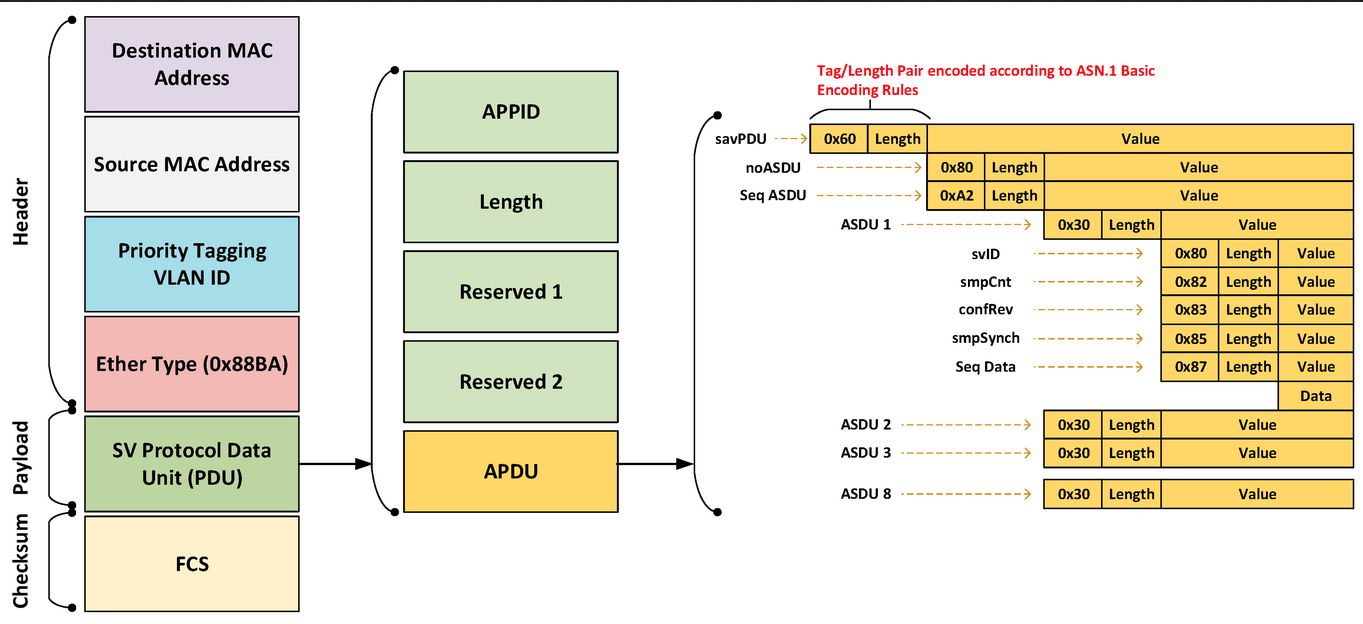
\includegraphics[width=0.95\textwidth, keepaspectratio]{ch5/assets/sv_packets_fields.png} % Reduce to 90% of the text width
\caption{Sampled Value packets fields. (Image credits: MDPI)}
\label{fig:sv_packet_fields}
\end{figure}
\FloatBarrier

Following the recommendations of \cite{uca2024guideline}, the description is well documented in \textcite[Subsection 4.2]{IEC61850_KTH}, which explains this in detail.


Figure~\ref{fig:Sv_packet_full} Here has a representation of all the field until the values, and all the layers of the packet. \cite{uca2024guideline}

\begin{figure}[tbh]
\centering
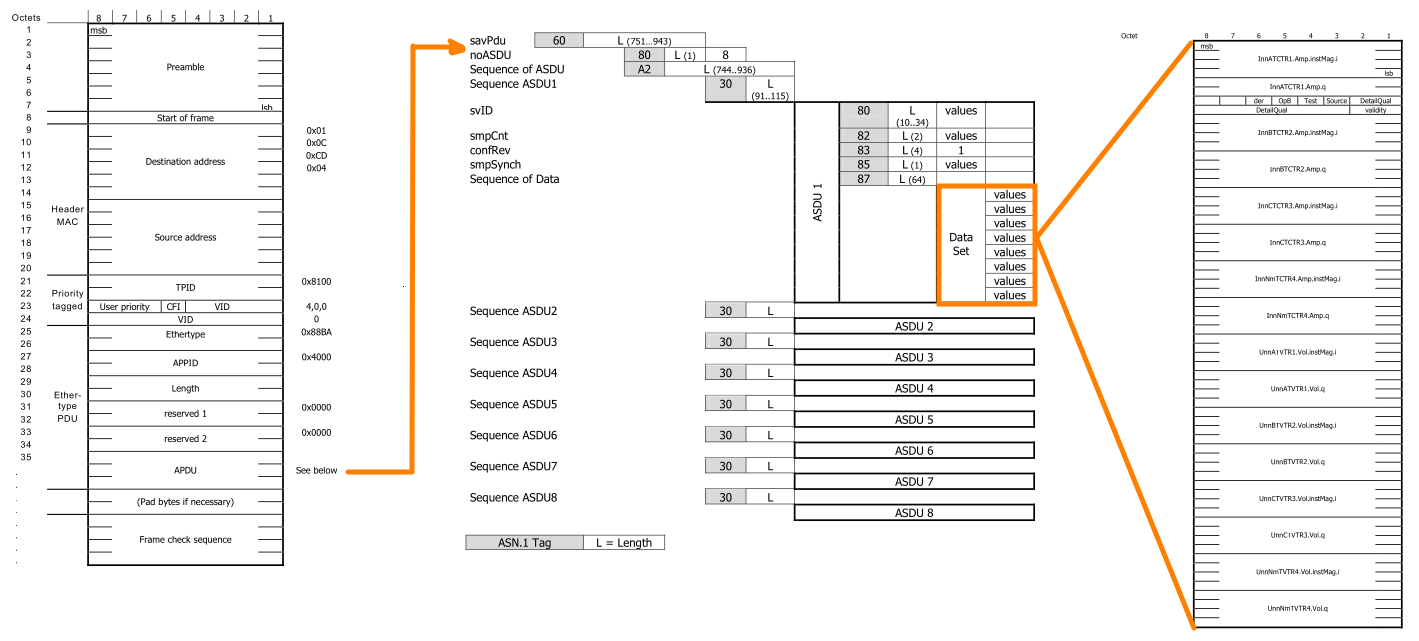
\includegraphics[width=0.95\textwidth, keepaspectratio]{ch5/assets/Sv_packet_full.png} % Reduce to 90% of the text width
\caption{Sampled Value packets fields. (Image credits: UCA International)}
\label{fig:Sv_packet_full}
\end{figure}
\FloatBarrier

\section{Development of a Publisher of IEC~61850-9-2-SV}

The development of the publisher is a critical component in the implementation of the IEC~61850-9-2 Sampled Values communication standard. This section outlines the structured approach taken to build the publisher, focusing on the creation of key data structures (structs) and the implementation of essential functions that enable the generation and transmission of SV packets.

\subsection{Structuring the Data: Defining Rust Structs}

The process begins with defining the necessary structs. Rust, known for its strong emphasis on safety and concurrency, offers a well-organized way to build and manage complex data structures. This allows for clear and readable code, where each step of the data flow is defined in a sequence that is easy to understand and maintain.

The primary structs used in this project are designed to mirror the components of an Ethernet frame, as required by the IEC~61850-9-2 standard. These structs are nested to represent the hierarchy of the data, from the Ethernet frame down to the individual data points in the SV payload.


\begin{lstlisting}[caption={Structs added}]
pub struct EthernetFrame
{
pub destination:    [u8; 6],
pub source:         [u8; 6],
pub tpid:           u16,
pub tci:            u16,
pub ethertype:      u16,
pub payload:        SvPDU,
pub fcs:            [u8; 4],
}

pub struct SvPDU
{
pub appid:          [u8; 2],
pub length:         [u8; 2],
pub reserved1:      [u8; 2],
pub reserved2:      [u8; 2],
pub apdu: SmvData,
}

pub struct SmvData
{
pub sav_pdu_asn:    [u8; 2],
pub no_asdu_asn:    [u8; 2],
pub no_asdu:        u8,
pub seq_asdu_asn:   [u8; 2],
pub asdu_asn:       [u8; 2],
pub sv_id_asn:      [u8; 2],
pub sv_id:          [u32; 1],
pub smp_cnt_asn:    [u8; 2],
pub smp_cnt:        [u16; 1],
pub conf_rev_asn:   [u8; 2],
pub conf_rev:       [u32; 1],
pub smp_synch_asn:  [u8; 2],
pub smp_synch:      u8,
pub seq_data:       [u8; 2],
pub logical_node: LogicalNode,
}

pub struct LogicalNode
{
pub i_a:    [i32; 1],
pub q_ia:   [u32; 1],
pub i_b:    [i32; 1],
pub q_ib:   [u32; 1],
pub i_c:    [i32; 1],
pub q_ic:   [u32; 1],
pub i_n:    [i32; 1],
pub q_in:   [u32; 1],
pub v_a:    [i32; 1],
pub q_va:   [u32; 1],
pub v_b:    [i32; 1],
pub q_vb:   [u32; 1],
pub v_c:    [i32; 1],
pub q_vc:   [u32; 1],
pub v_n:    [i32; 1],
pub q_vn:   [u32; 1],
}
\end{lstlisting}

These structs allow for a comprehensive representation of the Ethernet frame and the SV data contained within, ensuring that each element of the SV packet is accurately captured and can be easily manipulated during transmission.

\subsection{Implementing the Core Functions}

Once the data structures are in place, the next step is to implement the functions that will operate on these structs. Rust uses the 'impl' keyword to define methods for structs, allowing for the creation of constructors, data manipulation functions, and other essential operations.

For example, the implementation of a constructor for the 'EthernetFrame' struct might look like this:

\begin{lstlisting}[caption={How to implement an impl for the struct}]
/ Implementation of functions regarding EthernetFrame struct
impl EthernetFrame {
pub fn new(destination: [u8; 6], source: [u8; 6], tpid: u16, tci: u16, ethertype: u16, payload: SvPDU, fcs: [u8; 4]) -> Self {
Self {
	destination,
	source,
	tpid,
	tci,
	ethertype,
	payload,
	fcs,
}
}
\end{lstlisting}

This function allows for the creation of a new EthernetFrame instance, ensuring that all necessary fields are initialized correctly.

\subsection{Simulating an Electrical Grid Signal}

A key functionality of the publisher is to simulate the sinusoidal signal of an electrical grid. This simulation is essential for generating realistic SV packets that can be used to test and validate the SV communication system.

To achieve this, the current time is used as an input to calculate the voltage and current values, with predefined amplitudes representing the electrical parameters. This simulation is implemented in the following function:

\begin{lstlisting}[caption={How to calculate the value of the SV's }]
pub fn cal_current_phase_b ()-> [i32;1]
{
let now = Local::now();
let t: f32 = now.timestamp_subsec_nanos() as f32 / 1_000_000_000.0;
let phase_degrees: f32 = 120.0; // Example phase in degrees
let phase_radians: f32 = phase_degrees * PI / 180.0; // Convert phase to radians
let omega: f32 = 2.0 * PI * FREQUENCY;
let amplitude: f32 = AMPLITUDE_CURRENT * ((omega * t + phase_radians).sin());
[amplitude as i32;1]
}
\end{lstlisting}

This function calculates the current value for phase B at a given moment, using the system's local time to simulate the progression of the sinusoidal wave. The result is an array containing the current value, which can then be included in the SV packet.

\subsection{Introducing Invalid Samples for Testing}

To fully test the algorithm's ability to handle real-world scenarios, it was necessary to introduce invalid samples. This was accomplished by altering the quality of certain samples within the SV packets, making them invalid. The publisher was enhanced with a feature that allows these quality changes, enabling the testing of how well the algorithm can identify and respond to invalid data.

\begin{lstlisting}[caption={How to calculate the value of the SV's }]
if increment > 50 \&\& increment < 100
{
// Implement Bad Quality to the samples
// The value of 0 is good quality
// The value of 1 and 2 is invalid
//The value of 3 it is questionable
sv_packet.payload.apdu.logical_node.q_ia[0] = sv_packet.payload.apdu.logical_node.q_ia[0].wrapping_add(1);	
}
\end{lstlisting}

This method directly modifies the 'sv\_packet.payload.apdu.logical\_node.q\_ia' field, effectively marking the sample as invalid. This invalid data can then be used to test the robustness of the SV communication and processing algorithm.

\subsection{Finalizing the Publisher}

With the basic structure, implementation, and testing features in place, the development of the publisher was completed. The final publisher is capable of generating and transmitting SV packets, simulating electrical grid signals, and introducing invalid data for testing purposes. These features are critical to the overall success of the thesis, as they enable comprehensive testing and validation of the IEC~61850-9-2 SV standard.

\section{Development of a Subscriber of IEC~61850-9-2-SV}

The development process for the subscriber followed a similar structured approach as that of the publisher. Having already established the necessary structs during the publisher's development, the focus for the subscriber shifted towards receiving and processing the data transmitted by the publisher over the network.

In this context, the subscriber was designed to handle incoming Sampled Values (SV) packets, log the received data, and print the relevant information to the log. This approach not only facilitated real-time monitoring of the transmitted SV data but also provided a foundation for verifying the integrity and accuracy of the data exchange between the publisher and subscriber.

\subsection{Structs Reused in the Subscriber}

Given that the subscriber's primary role is to interpret the data sent by the publisher, the same set of structs, including 'EthernetFrame', 'SvPDU', 'SmvData', and 'LogicalNode', were reused. These structs allowed the subscriber to decode the incoming Ethernet frames and extract the necessary information from the SV packets.

\begin{lstlisting}[caption={EthernetFrame struct. }]
	pub struct EthernetFrame {
		pub destination: [u8; 6],
		pub source: [u8; 6],
		pub tpid: u16,
		pub tci: u16,
		pub ethertype: u16,
		pub payload: SvPDU,
		pub fcs: [u8; 4],
}

// Other structs reused as shown in the publisher's code...
\end{lstlisting}

\subsection{Implementation of Data Reception and Logging}

The implementation phase involved creating functions to capture the network packets, parse them into the appropriate struct fields, and log the data for analysis. The impl blocks provided a seamless way to define these methods, ensuring that the subscriber could efficiently process the data.

\subsection{Error Handling and Invalid Data Processing}

An essential part of the subscriber’s functionality involved handling errors and invalid data. Similar to the publisher, where invalid samples were introduced to test the algorithm, the subscriber needed to identify and appropriately respond to these invalid samples. This was achieved by checking the quality of the received data and ensuring that any invalid samples were flagged and processed correctly.

\subsection{Finalizing the Subscriber}

By incorporating robust data reception, validation, and logging mechanisms, the subscriber was completed with the essential features required to support the overall thesis objectives. The subscriber was now fully equipped to interact with the publisher, process the received SV packets, and handle any errors or invalid data that might arise during transmission. This setup provided a solid foundation for testing and verifying the performance of the implemented communication protocol.
